\documentclass{article}
\usepackage{multicol}
\usepackage{geometry}
\usepackage{blindtext}
\usepackage[sort, numbers]{natbib}

%\renewcommand{\familydefault}{\sfdefault}
%\usepackage{helvet}
\setlength{\columnsep}{1cm}
%\setlength{\columnseprule}{0.4pt}
\setlength{\footskip}{20pt}
\usepackage{fancyhdr}
\usepackage{hyperref}
\fancyhf{}
\fancyhead[C]{FetalMed-PhD $\bullet$ PhD Proposal $\bullet$ Joe Brew}
\fancyfoot[C]{  $\bullet$ joebrew@gmail.com $\bullet$  }
\renewcommand\headrulewidth{1pt}

\pagestyle{fancy}



\usepackage{Sweave}
\begin{document}
\Sconcordance{concordance:protocol.tex:protocol.Rnw:%
1 22 1 1 0 31 1 1 9 1 3 81 1 1 9 1 1 1 77 1 1 1 12 1 2 75 1}


\newgeometry{margin=2.5cm}



\begin{center}

\rule{\textwidth}{1.6pt}\vspace*{-\baselineskip}\vspace*{2pt} % Thick horizontal line
\rule{\textwidth}{0.4pt}\\[\baselineskip] % Thin horizontal line


\begin{LARGE}
\scshape{detection of geographical clusters of prematurity and low birth weight in an urban area}
\end{LARGE}

\rule{\textwidth}{0.4pt}\vspace*{-\baselineskip}\vspace{3.2pt} % Thin horizontal line
\rule{\textwidth}{1.6pt}\\[\baselineskip] % Thick horizontal line

\vspace{10mm}

\begin{Large}
Joe Brew
\end{Large}
\vspace{3mm}

\begin{large}
Erasmus Mundus, FetalMed PhD Proposal 
\end{large}

\vspace{20mm}
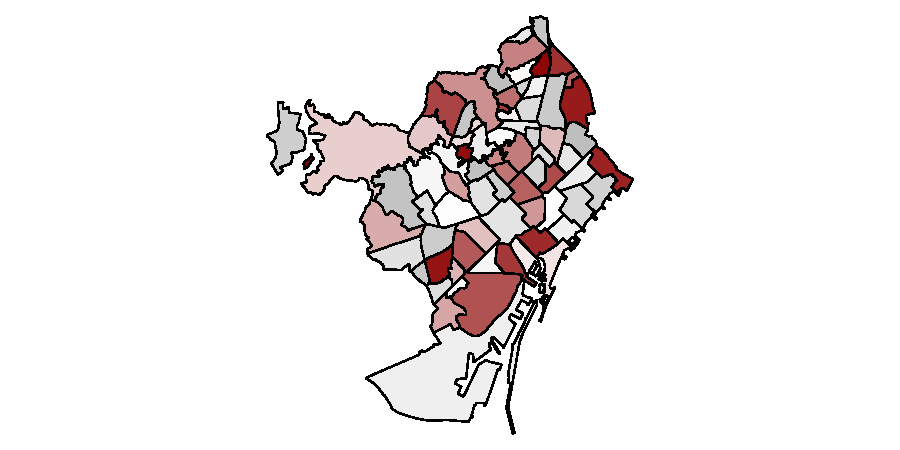
\includegraphics{protocol-001}

\vspace{20mm}


\subsection*{Project summary}

\end{center}



\noindent \emph{Though clinical treatments for infants born prematurely and/or at low weight have improved, there is an urgent need for research into these adverse events' causes.  Of particular need is a framework for identifying and understanding prematurity and low weight birth's spatial components, so as to direct preventive health interventions.  Using spatial statistics and novel machine learning methods, this project aims to develop a framework through which Barcelona can identify clusters indicative of adverse prenatal health exposures, and then expand that framework to other European cities.} 


\newpage

\begin{multicols}{2}
\setkeys{Gin}{width=0.5\textwidth}



\subsection*{General information}

\noindent \textbf{Project:}\\ Detection of geographical clusters of prematurity and low birth weight in an urban area \\

\noindent \textbf{Investigators:} \\ Joe Brew, MPH, MA (applicant) \\ Montse Palacio, MD (requested supervisor) \\


\noindent \textbf{Research questions:}\\ What factors affect the likelihood of premature birth and low birth weight in Barcelona, Spain?  After adjustment for relevant sociodemographic confounders, can geographic information system (GIS) tools and spatial statistics be used to predict cases of premature birth and low birth weight?  To what extent do environmental exposures explain spatially differential risk? How can municipal public health authorities intervene to prevent adverse birth outcomes in high-risk areas? Can models and methods devised for prediction in Barcelona be applied in other Spanish and European cities?    \\

\noindent \textbf{Importance / Rationale:}\\  In the first moments of life, preterm and low birth weight (LBW) infants are at a greater risk of neonatal mortality \cite{Tsai2014,Anderson2014} and morbidity \cite{Yeung2014,Merkestein2014}.   When these infants survive, they face a higher likelihood of chronic conditions as adults \cite{Visentin2014,Lane2014}.  \\ 

\noindent There is a growing body of research into the negative \emph{consequences} of prematurity, and a greater push for newborn-specific interventions to reduce neonatal mortality. \cite{Eichenwald2008, Wardlaw2014} However, there is a lack of research into its \emph{causes}, particularly in regards to prevention, \cite{GrisaruGranovsky2014,Rubens2014}.  Social and demographic risk factors have been established \cite{Slopen2015, Yego2014}, but many of them are not "intervenible" \cite{Schempf2007, Shah2010, Kozuki2013}. Recent technological advances have enabled better clinical detection methods \cite{Hatanaka2014, Wapner2014}, but detection does not, in itself, \emph{prevent}. \\

\noindent Environmental exposures, particularly the inhalation of fine particulate matter and residing in areas with air pollution , have been identified as an important intervenible risk factor for prematurity and LBW both in Spain \cite{2014} and internationally \cite{Yorifuji2015, Morales2014, deMelo2014}. However, most environmental studies are carried out at an aggregated level, and do not account for variation in level of exposure within urban areas. These studies, though useful to national-level authorities, are of little value to local and regional-level public health practitioners.  An understanding of environmental exposures at the local level is essential to primary prevention, and the first step in identifying these exposures is the identification of spatial clusters.  \\

\noindent As with clinical screening methods, tools for epidemiological investigation and geospatial analysis have improved rapidly in recent years.  This project combines needed research into an area of relative uncertainty (differential risk by neighborhood) with modern tools (GIS) and methods (krieging, Moran's I, LISA, random forests, spatial scans, clustering detection, etc.), so as to better understand a problem of significant public health importance.


\subsection*{Study objectives}
The objectives of this project are two-fold: 
\begin{enumerate}
\item Identify both spatial and non-spatial risk factors for LBW and premature birth in the city of Barcelona, Spain, using novel machine learning approaches and GIS tools, with a focus on prenatal environmental exposures at the neighborhood level.
\item Given the results of the first objective, test the model's predictive ability on non-Barcelona data, and design an intervention framework for the prevention of LBW and prematurity for European cities. 
\end{enumerate}


\subsection*{Study Design}
\noindent \textbf{Design:} Prospective, observational cohort study \\

\noindent \textbf{Research population:} Expectant mothers in their first or second trimester residing in Barcelona, Spain during the study recruitment time period. \\

\noindent \textbf{Time period:} Study participants will be recruited from October, 2015 through March, 2016.  


\subsection*{Methodology}

\noindent \textbf{Data acquisition and organization:} Following approval from the appropriate ethical committees, institutional review boards, and governmental agencies, pregnant women in their first or second trimesters of pregnancy will be recruited to participate in the study.  "Participation" constitutes (a) a simple 5-10 minute survey outlining basic socioeconomic, demographic and medical traits/history as well as residential, family and labor market information and (b) agreement to allow access to their birth outcome data (gestional age, weight at birth, survival and defects status). \\

\noindent \textbf{Exclusion criteria:} Given the simplicity of the survey and lack of any risk for participants, there are no explicit exclusion criteria in the data collection phase.  In the analysis phase, subjects may be excluded given certain pre-existing health conditions or non-representative demographic traits.   \\

\subsection*{Safety Considerations}

There are no reasonable foreseeable safety considerations associated with this research.  


\subsection*{Data Management and Statistical Analysis}

\noindent \textbf{Data management:} Private health data will be stored on a password-protected and fully encrypted hard-drive, and will accessed locally only by the principal investigators.  Following initial collection and cleaning, data will be "anonymized" by using unique key-pairs (ID numbers linked to mother's name), stored in a separate linkage document to which only the principal investigators have access. \\ 

\noindent \textbf{Statistical analysis:} The analysis phase of the project has three phases: \begin{enumerate}
\item Feature generation, aggregation and public data joins
\item Model construction 
\item Model testing
\end{enumerate}

In phase 1, the dataset constructed through the surveying and birth outcomes collection will be joined to Spanish census data as well as relevant commercial and infrastructure data (proximity to major roads, industrial sites, etc.). Additionally, study participants will be stratified into risk "groups" based on established non-spatial risk factors for LBW and premature birth. \\

In phases 2 and 3, analysis will take a typical machine learning approach to variable/model selection and validation.  Statistical models will be constructed with the aim of predicting the likelihood of both prematurity and LBW given a combination of relevant spatial and non-spatial features.  6 different model types (logistic regression, generalized additive model, krieging, Kulldorff's spatial scan, random forest, and support vector regression) will be "trained" on a randomly selected subset (constituting two thirds of the total number of study participants), and then "tested" on the remaining third's outcomes.  Model strengths, weaknesses and extrapolatability will be explored through standardized tests. \\

\noindent \textbf{Data deliverable:} Finally, by standardizing non-spatial features, risk by neighborhood (left) as well as a spatial risk "surface" for the entirety of Barcelona's municipal area (right) can be constructed (both examples using simulated data).  This will be useful both to public health practitioners (who can identify neighborhoods of greatest risk, and therefore greatest need) as well as to the research community at large. 





\begin{center}
\includegraphics{protocol-004}
\end{center}




\noindent \textbf{Research Deliverables: Dissemination of Results and Publication Policy}

This study has both scientific (objective 1) and policy (objective 2) components.  For the former, results will be published in academic journals, with credit attributed to the relevant universities, governmental agencies and Erasmus Mundus organization.  For the latter, the main objective is the development and dissemination of a predictive framework applicable to other European cities.  This "framework" consists of both a "toolkit" (open-source statistical code) as well as an interactive web component to help guide public health practitioners in the identification of LBW and prematurity clusters in their own cities.  

\subsection*{Expected Outcomes of the Study}

Given the established importance of environmental factors to maternal and infant health outcomes, it is reasonable to foresee the identification of "clusters" which cannot be fully explained by their non-spatial components. 

\subsection*{Duration of the Project}

In general terms, the first year of the project will consist of survey and study design refinement, the second year will consist of data cleaning, feature generation and analysis, and the third year will be devoted to publication, dissemination and the construction of the European cities' "toolkit."  

\subsection*{Problems Anticipated}

None.

\subsection*{Project Management}

This project will be carried out in accordance with the regulations and guidelines of the Erasmus Mundus and FetalMed PhD programs, under the direction of Montse Palacio (the requested project director), with the principal research being carried out by Joe Brew (the PhD applicant). 

\subsection*{Ethics}

Mr. Brew will seek approval from the relevant committees, conforming both to the guidelines of law as well as best practice.


\subsection*{Informed consent}
Informed consent will be provided in the form of a letter as well as the attending physician's explanation.  The letter will be available in Catalan, Spanish, French, English, Portuguese, Arabic and Turkish.  For potential participants who do not read, or who do not understand the aforementioned languages, a medical interpretor will be sought both for the purposes of the visit, as well as the translation of the letter of informed consent.  Participants will be asked to sign to signify their agreement with the study terms.  A participant may remove themselves from the study upon simple request at any point in the data collection or analysis phases.  There are no incentives or de-incentives for study participation.  


\subsection*{Budget}

The budget for this project will be minimal, and incidental costs (printing, computing, etc.) will be incurred by Mr. Brew.  

\subsection*{Other support for the Project}

Mr. Brew seeks a Category A Erasmus Mundus grant for the purposes of this project.

\subsection*{Collaboration with other scientists or research institutions}

Particularly in the accomplishment of objective 2 (the construction of a predictive framework for LBW and premature birth for other European cities), collaboration will be a necessary component of this project.  

\subsection*{Credentials of the investigators}

Mr. Brew is an experienced data scientist and public health practitioner.  He currently works as the surveillance epidemiologist for the Florida Department of Health in Alachua County.  His work for FDOH has focused on low birth weight, infant mortality, and geography.  He has previously worked as a "Data Science for Social Good" fellow with the Chicago Department of Public Health, where he developed a predictive model to identify lead poisoning cases among infants and children. \\

Dr. Palacio, Maternal-Fetal consultant and Chair of the Obstetric and High Risk Obstetrics wards at the Hospital Universitari, is an expert in the field of fetal medicine.  Her combination of subject matter and clinical experience, as well as her familiarity with Barcelona's clinical and data systems, are essential to this projects success.  


\subsection*{Format}
This protocol follows the \href{http://www.who.int/rpc/research_ethics/format_rp/en/}{format recommended by the World Health Organization}. \\

\subsection*{Contact}
Joe Brew, MPH, MA\\
530 NW 2nd Street \\
Gainesville, FL 32601 \\
USA \\
352.318.4553 \\
joebrew@gmail.com

\end{multicols}
\setkeys{Gin}{width=1\textwidth}
%----------------------------------------------------------------------------------------
%  REFERENCE LIST
%----------------------------------------------------------------------------------------
\newpage
\bibliographystyle{unsrtnat}
\bibliography{test}



\end{document}
